% Submission-facing vector figures. Numerical coordinates are frozen/publication evidence.

\newcommand{\figSystemArchitecture}{%
\begin{figure*}[t]
\centering
\resizebox{\textwidth}{!}{%
\begin{tikzpicture}[font=\footnotesize, node distance=7mm and 8mm,
box/.style={draw, rounded corners, align=center, minimum height=8mm, minimum width=27mm, fill=black!3},
smallbox/.style={draw, rounded corners, align=center, minimum height=7mm, minimum width=24mm, fill=black!2},
arr/.style={-Latex, thick}]
\node[box] (state) {Physical / estimated state\\$E_b/N_0$, IF-SNR, $R$, $v$, CFO, INR};
\node[box, right=of state] (gate) {Deterministic\\physics gate};
\node[box, right=of gate] (actions) {Feasible subset of\\54 PC-FMCW actions};
\node[box, right=of actions] (unc) {Action-local\\uncertainty draws};
\node[box, right=of unc] (wilson) {Joint-QoS test +\\Wilson lower bound};
\node[box, right=of wilson] (select) {Minimum-cost accepted\\action or abstention};
\node[smallbox, below=of select, xshift=-17mm] (comm) {Communication receiver\\DBPSK / BER / rate};
\node[smallbox, below=of select, xshift=17mm] (radar) {Sensing receiver\\dechirped IF / $R,v$ RMSE};
\draw[arr] (state) -- (gate);
\draw[arr] (gate) -- node[above]{hard support} (actions);
\draw[arr] (actions) -- (unc);
\draw[arr] (unc) -- (wilson);
\draw[arr] (wilson) -- (select);
\draw[arr] (select) -- (comm);
\draw[arr] (select) -- (radar);
\end{tikzpicture}%
}
\caption{Physics-gated reliability-constrained PC-FMCW adaptation. Hard range/velocity representability is checked before stochastic reliability qualification. B4 accepts an action only if the one-sided Wilson lower bound for the joint-QoS success event reaches the frozen reliability target; otherwise it abstains.}
\label{fig:architecture}
\end{figure*}}

\newcommand{\figFrozenPolicies}{%
\begin{figure*}[t]
\centering
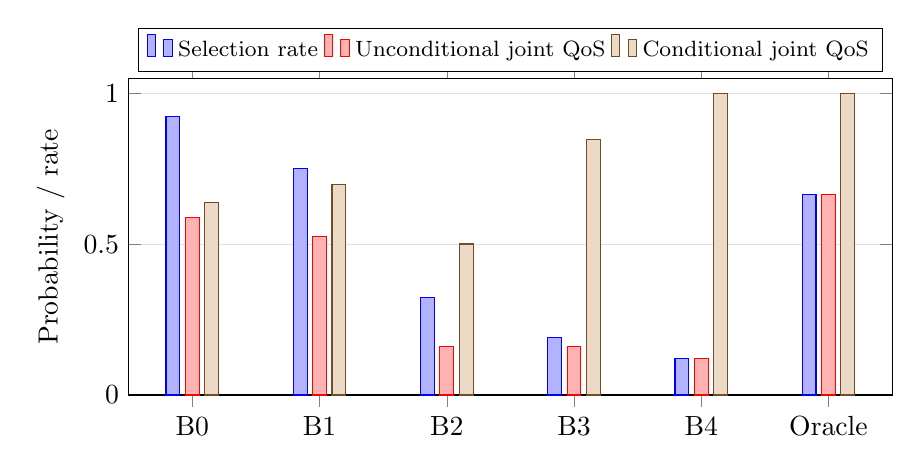
\begin{tikzpicture}
\begin{axis}[
width=0.93\textwidth,height=5.6cm,
ybar,bar width=5pt,
ymin=0,ymax=1.05,
ylabel={Probability / rate},
symbolic x coords={B0,B1,B2,B3,B4,Oracle},xtick=data,
legend style={at={(0.5,1.02)},anchor=south,legend columns=3,font=\footnotesize},
major grid style={black!12},ymajorgrids=true,
]
\addplot coordinates {(B0,0.9235833)(B1,0.7531667)(B2,0.3225833)(B3,0.1906667)(B4,0.1223333)(Oracle,0.6666667)};
\addplot coordinates {(B0,0.5904167)(B1,0.5259167)(B2,0.16175)(B3,0.16175)(B4,0.1223333)(Oracle,0.6666667)};
\addplot coordinates {(B0,0.6392673)(B1,0.6982740)(B2,0.5014208)(B3,0.8483392)(B4,1.0)(Oracle,1.0)};
\legend{Selection rate,Unconditional joint QoS,Conditional joint QoS}
\end{axis}
\end{tikzpicture}
\caption{Frozen v2.1 paired benchmark over 12,000 state/seed units per policy. B4 has the highest observed selected-case reliability among deployable policies but the lowest availability among the adaptive joint policies; its unconditional joint-QoS probability is lower than B3.}
\label{fig:frozen-policies}
\end{figure*}}

\newcommand{\figUncertaintyTradeoff}{%
\begin{figure}[t]
\centering
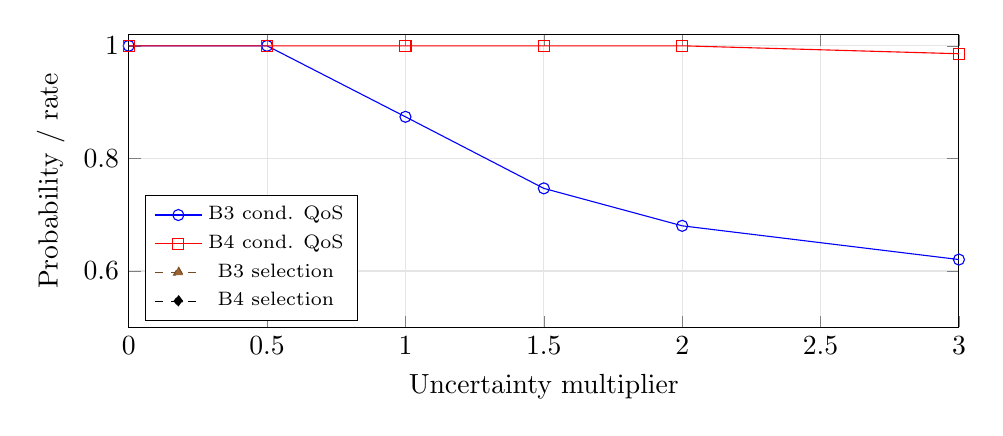
\begin{tikzpicture}
\begin{axis}[
width=\columnwidth,height=5.3cm,
xlabel={Uncertainty multiplier},ylabel={Probability / rate},
xmin=0,xmax=3,ymin=0.5,ymax=1.02,
legend style={font=\scriptsize,at={(0.02,0.02)},anchor=south west},
grid=major,major grid style={black!10}]
\addplot+[mark=o] coordinates {(0,1)(0.5,1)(1,0.8739)(1.5,0.7468)(2,0.6803)(3,0.6204)};
\addplot+[mark=square] coordinates {(0,1)(0.5,1)(1,1)(1.5,1)(2,1)(3,0.9859)};
\addplot+[mark=triangle*,dashed] coordinates {(0,0.1667)(0.5,0.1667)(1,0.185)(1.5,0.1975)(2,0.2033)(3,0.2283)};
\addplot+[mark=diamond*,dashed] coordinates {(0,0.1667)(0.5,0.1617)(1,0.125)(1.5,0.1117)(2,0.0975)(3,0.0592)};
\legend{B3 cond. QoS,B4 cond. QoS,B3 selection,B4 selection}
\end{axis}
\end{tikzpicture}
\caption{Supplemental uncertainty sweep. Increasing uncertainty makes B4 progressively more selective while preserving higher conditional joint-QoS probability; at multiplier 3, however, B4's one-sided Wilson lower bound falls below the declared 0.95 target despite the 0.9859 point estimate.}
\label{fig:uncertainty-tradeoff}
\end{figure}}

\newcommand{\figFiniteDrawCalibration}{%
\begin{figure}[t]
\centering
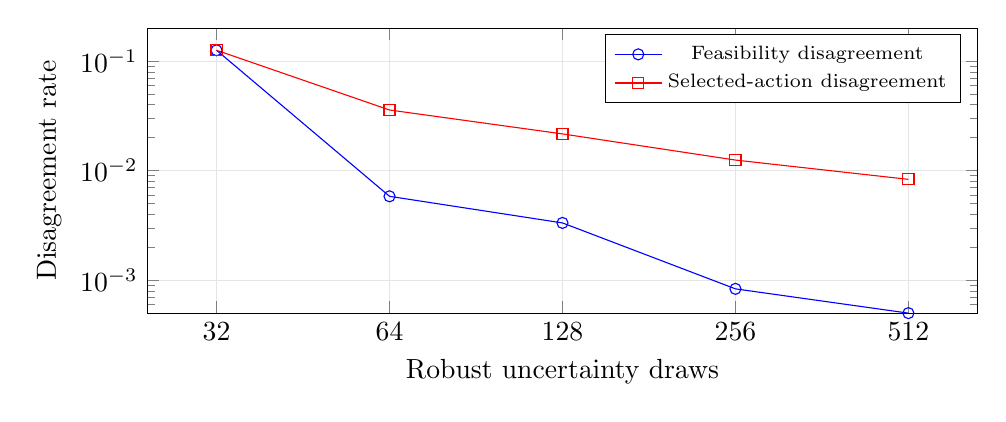
\begin{tikzpicture}
\begin{semilogyaxis}[
width=\columnwidth,height=5.2cm,
xlabel={Robust uncertainty draws},ylabel={Disagreement rate},
xmode=log,log basis x=2,
ymin=5e-4,ymax=0.2,
xtick={32,64,128,256,512},xticklabels={32,64,128,256,512},
legend style={font=\scriptsize,at={(0.98,0.98)},anchor=north east},
grid=major,major grid style={black!10}]
\addplot+[mark=o] coordinates {(32,0.125833)(64,0.005833)(128,0.003333)(256,0.000833)(512,0.0005)};
\addplot+[mark=square] coordinates {(32,0.125833)(64,0.035833)(128,0.021667)(256,0.0125)(512,0.008333)};
\legend{Feasibility disagreement,Selected-action disagreement}
\end{semilogyaxis}
\end{tikzpicture}
\caption{Finite-draw calibration against the nested 4096-draw Monte-Carlo reference. The plotted 512-draw feasibility value is shown at $5\times10^{-4}$ only to visualize the observed zero on a log axis; the measured feasibility disagreement is exactly 0, while selected-action disagreement remains 0.833\%.}
\label{fig:finite-draw}
\end{figure}}

\newcommand{\figRuntimeScaling}{%
\begin{figure}[t]
\centering
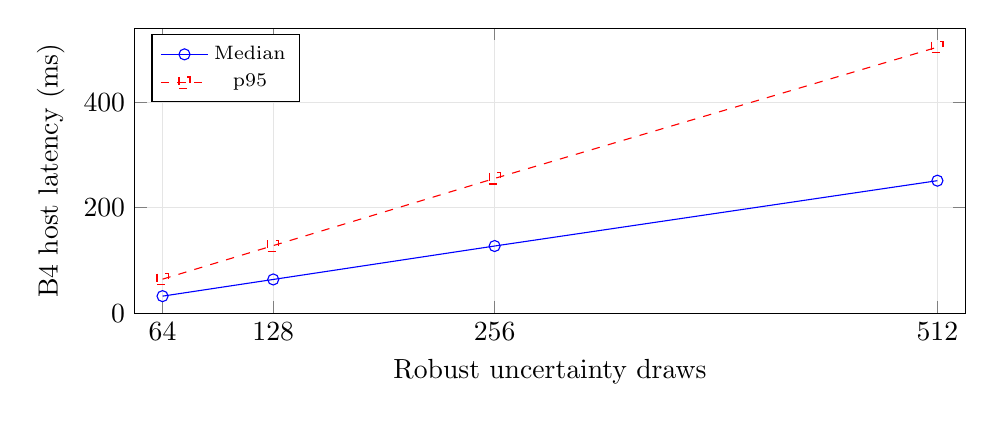
\begin{tikzpicture}
\begin{axis}[
width=\columnwidth,height=5.2cm,
xlabel={Robust uncertainty draws},ylabel={B4 host latency (ms)},
xmin=48,xmax=528,ymin=0,ymax=540,
xtick={64,128,256,512},
legend style={font=\scriptsize,at={(0.02,0.98)},anchor=north west},
grid=major,major grid style={black!10}]
\addplot+[mark=o] coordinates {(64,32.17)(128,63.81)(256,127.19)(512,251.04)};
\addplot+[mark=square,dashed] coordinates {(64,64.37)(128,127.98)(256,255.28)(512,504.11)};
\legend{Median,p95}
\end{axis}
\end{tikzpicture}
\caption{Host-runtime scaling for B4 in the final reviewer-grade evidence. The near-linear growth with uncertainty draws quantifies the computational cost of stronger Monte-Carlo qualification. These are Python/Linux host timings, not embedded-ECU measurements.}
\label{fig:runtime}
\end{figure}}
